\section{The 555 Timer (and Friends)}
\label{lab_timers}

%\makelabheader %(Space for student name, etc., defined in master.tex)

\bigskip

If you were trapped on a desert island and could have only a single integrated circuit with you, what would you choose?  One good answer is the 555 timer, which consists of two comparators and one flip-flop, plus a few extra internal resistors and an output stage to increase its utility.  As the block diagram below suggests, 555 timers can do anything that flip-flops or comparators can do alone, but they often simplify your circuit by requiring fewer external components. 

%\begin{center}
%\vspace{-0.05in}
%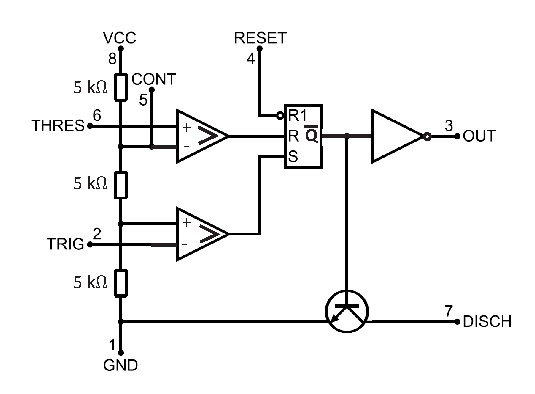
\includegraphics[width=3.25in]{timers/555_block_diagram.eps}
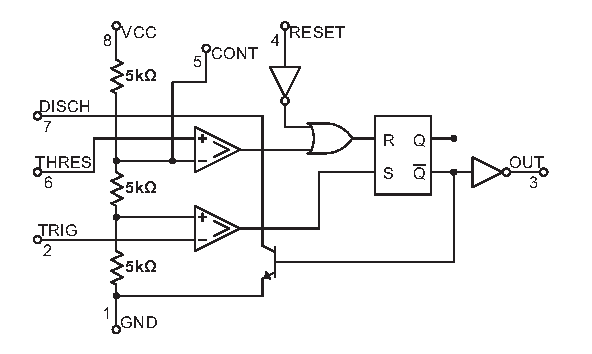
\includegraphics[scale=0.96]{timers/555_block_diagram_multisim.eps}
\hspace{-0.7in}
\hfill
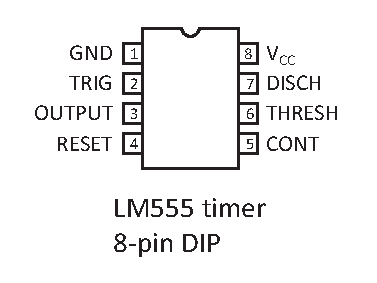
\includegraphics[scale=0.72]{timers/lm555_simple_2line.eps}
\hspace{-0.2in}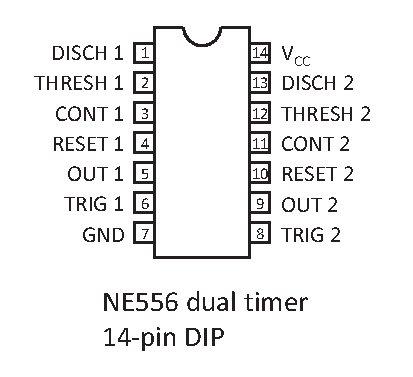
\includegraphics[scale=0.72]{timers/ne556_abrev_2line.eps}
\hspace{-0.1in}
%\vspace{-0.05in}
%\end{center}

The 555 timer was first developed in 1971, and is still selling over a billion chips per year.  The original was the NE555 made by Signetics, but it is now made by many  manufacturers and in countless variations (for high speed, low power, low voltages, extreme temperatures, etc.).  It also comes in versions with two or even four devices on one chip.  The pinouts for two common versions are shown above.  In this lab, we'll consider three common uses for this best-selling chip of all time. 

\begin{enumerate}[wide]

\item \textbf{Bistable mode}: When wired as shown below, the circuit acts like a simple flip-flop (but without the fancy clock and data inputs that you get with a chip like the CD4013).  The inputs are normally held high at $V_{CC}$.  When the trigger input is momentarily brought to ground, the output swings to $V_{CC}$ and stays there.  
%When the reset is momentarily brought to ground, the output swings to 0~V and stays there.  
What happens when the reset is momentarily brought to ground?
(Although the CONTROL input is not specifically used in this application, it is common nevertheless to place a 10~nF capacitor between CONTROL and ground, to reduce unwanted interference.)  
%[Test this to see what happens when inputs are held open...]  
\begin{center}
\vspace{-0.15in}
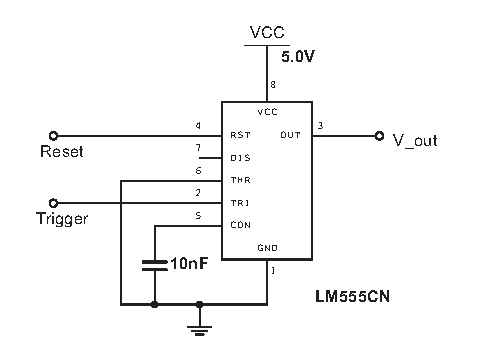
\includegraphics{timers/bistable_555.eps}
\vspace{-0.05in}
\end{center}

\pagebreak[3]
\item \textbf{Monostable mode}: In this mode, the 555 acts as a ``one shot'' timer.  When a trigger signal is given, the output signal jumps from 0 to $V_{CC}$ for a time given by 
$$\Delta t = \ln (3) RC \approx 1.1 RC.$$
The output then resets to zero and waits for another trigger event.  The trigger in this case happens when the input signal at the TRIG input falls below a certain fraction of $V_{CC}$.  What fraction would that be, by the way?  You should be able to tell by looking at the block diagram of the chip, especially those three 5~k$\Omega$ resistors in series.  Make a prediction, then build the circuit to test it out.  Aim for a delay time of $\Delta t \approx 3$~seconds.
\begin{center}
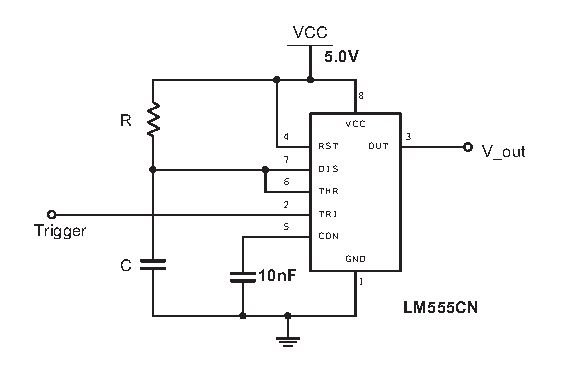
\includegraphics{timers/monostable_555.eps}
\end{center}

\item \textbf{Astable mode}: In this mode, the 555 acts as a square wave generator, much like the one you built using a single comparator in Lab~\ref{lab_capacitors}, part \ref{part_square_generator}.  In the circuit shown below, when the output swings high to $V_{CC}$, the capacitor $C$ charges through $R_1$ and $R_2$.  When the output swings low, the discharge lead (pin 7) is pulled to 0~V, and the capacitor discharges through $R_2$ only.  Because of this, the square wave produced by this circuit is asymmetric, with the dwell times given by
%$$
\begin{align*}
\Delta t_{HIGH} &= \ln (2) C(R_1 + R_2) \textrm{, and} \\
\Delta t_{LOW} &=\ln (2) CR_2.
\end{align*}
%$$
Build the circuit below, choosing values for $R_1$, $R_2$, and $C$ that will yield a square wave with a ratio of 
$\Delta t_{HIGH} / \Delta t_{LOW} =2$, and a frequency of $f \approx 10$~kHz. \label{part_astable}
\begin{center}
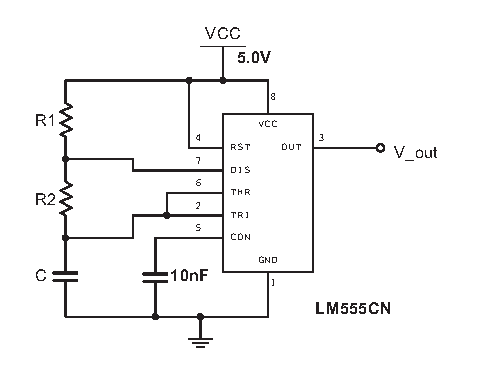
\includegraphics{timers/astable_555.eps}
\end{center}

\item The ``duty cycle'' of a square wave is the percentage of each cycle that the output is at a high voltage.  If you want to make a square wave with a duty cycle of less than 50\%, there's a neat trick you can use to make the capacitor charge faster than it discharges: place a diode in parallel with $R_2$, oriented so that $R_2$ is effectively shorted out during the charging phase.  Modify your previous circuit so that the output pulse has a duty cycle of about 20\%.  (Don't worry about its frequency, just get the duty cycle close.)

\item Use a single 556 timer chip (two timers on the same IC) to build a beeper that beeps a warning at about 1~kHz.  The beeper should sound on and off about once per second.  For this, you'll want to have one 1~Hz oscillator that effectively turns a second 1~kHz oscillator on and off every second.  Looking at the circuit diagram in part~\ref{part_astable}, what's a good way to turn your oscillator on and off without cutting power to the entire chip?

\item You probably noticed that the pitch of your beeper sounds a little unsteady.  What's happening is that because of the low impedance of the speaker, the high current drawn from the 556 timer is causing some change in its performance, perhaps due to internal heating.  To fix this problem, use a single MJE3055T transistor as an emitter follower amplifier between the 556 timer and the speaker.  The pin-out diagram of the MJE3055T is shown in Appendix~\ref{appendix_pinouts}.  Draw a diagram showing how to wire this up, and build it to confirm that it works as expected.
\end{enumerate}







